\section{State of the Art}

State of the art is the level of knowledge and development achieved in a technique,science, etc, esp at present (dictionary.com - SOTA). Regarding this project SOTA will be analysis of similar applications and if and how they use mobile sensors or any other non traditional mobile interaction at present.  Analysing and understanding SOTA will help to build “on-top” of what market offers to create better app. 

\subsection{Similar applications on market} 
\subsubsection{IKEA kitchen planner}
IKEA offers two applications to plan furniture placing in customers homes. The first one goes after the name “IKEA kitchen planner”. In this application customers can create accurate measurements of their own kitchen and place the furniture from IKEA’s catalogue. It is possible to do different wall measurements, add wallpapers to walls, apply different ceiling and floor covers, add windows and doors. Users can view the layout from top-down view and later see how furnitured layouts look in 3D perspective.
Users have a possibility to browse IKEA’s furniture on sale and add it to their designed rooms.
Pictures below show the application’s appearance: 1 - top-down layout, 2 - layout with placed furniture, 3 - 3D representation.

\begin{figure}[H]
\centering
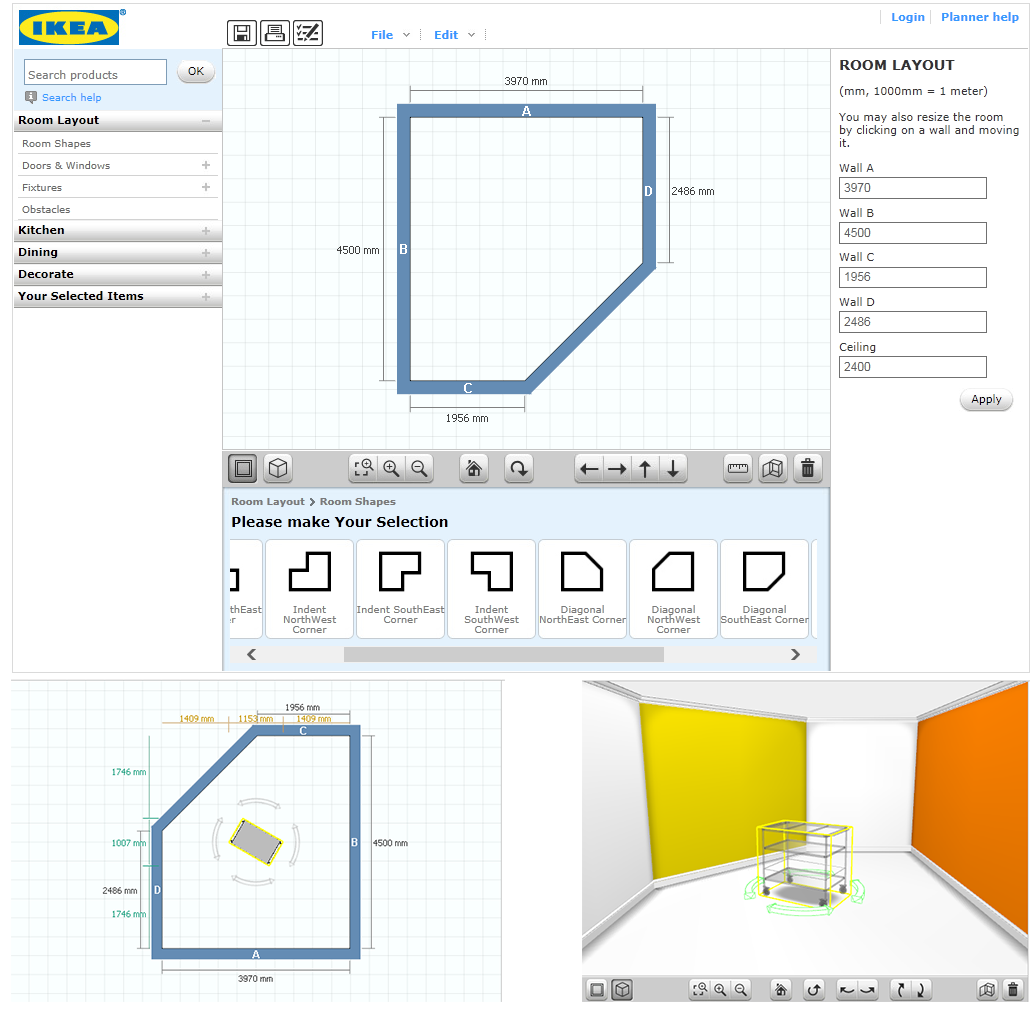
\includegraphics[scale=0.3]{kitchen1.png}
\caption{IKEA’s kitchen planning application}
\end{figure}


The application is rich in features. It offers short description, dimensions and price of each item that is on sale. It is possible to accurately rotate and place any chosen item. The items do not overlap unrealistically - the designing of the room gives realistic outcomes. There are also “smart” helping features such as snapping the items to the wall or to a specifically selected place. For instance - if the user wants to replace an item with another one, they automatically switch places.
.
\begin{figure}[H]
\centering
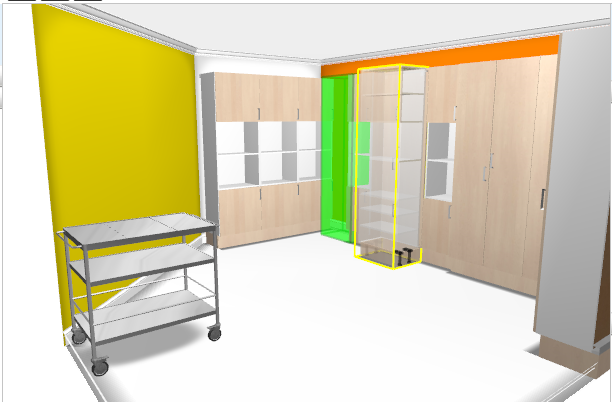
\includegraphics[scale=0.3]{kitchen2.png}
\caption{IKEA’s kitchen planning app}
\end{figure}

User has the possibility to log in and save the layout and check overall price status of items added to the room.

However this application is built for PC and not for mobile platforms. It takes some time to get used to it as the application is vast and rich in features. Some of the IKEA’s centers have dedicated PC rooms with assistant employees that help users navigate this application. 

\begin{figure}[H]
\centering
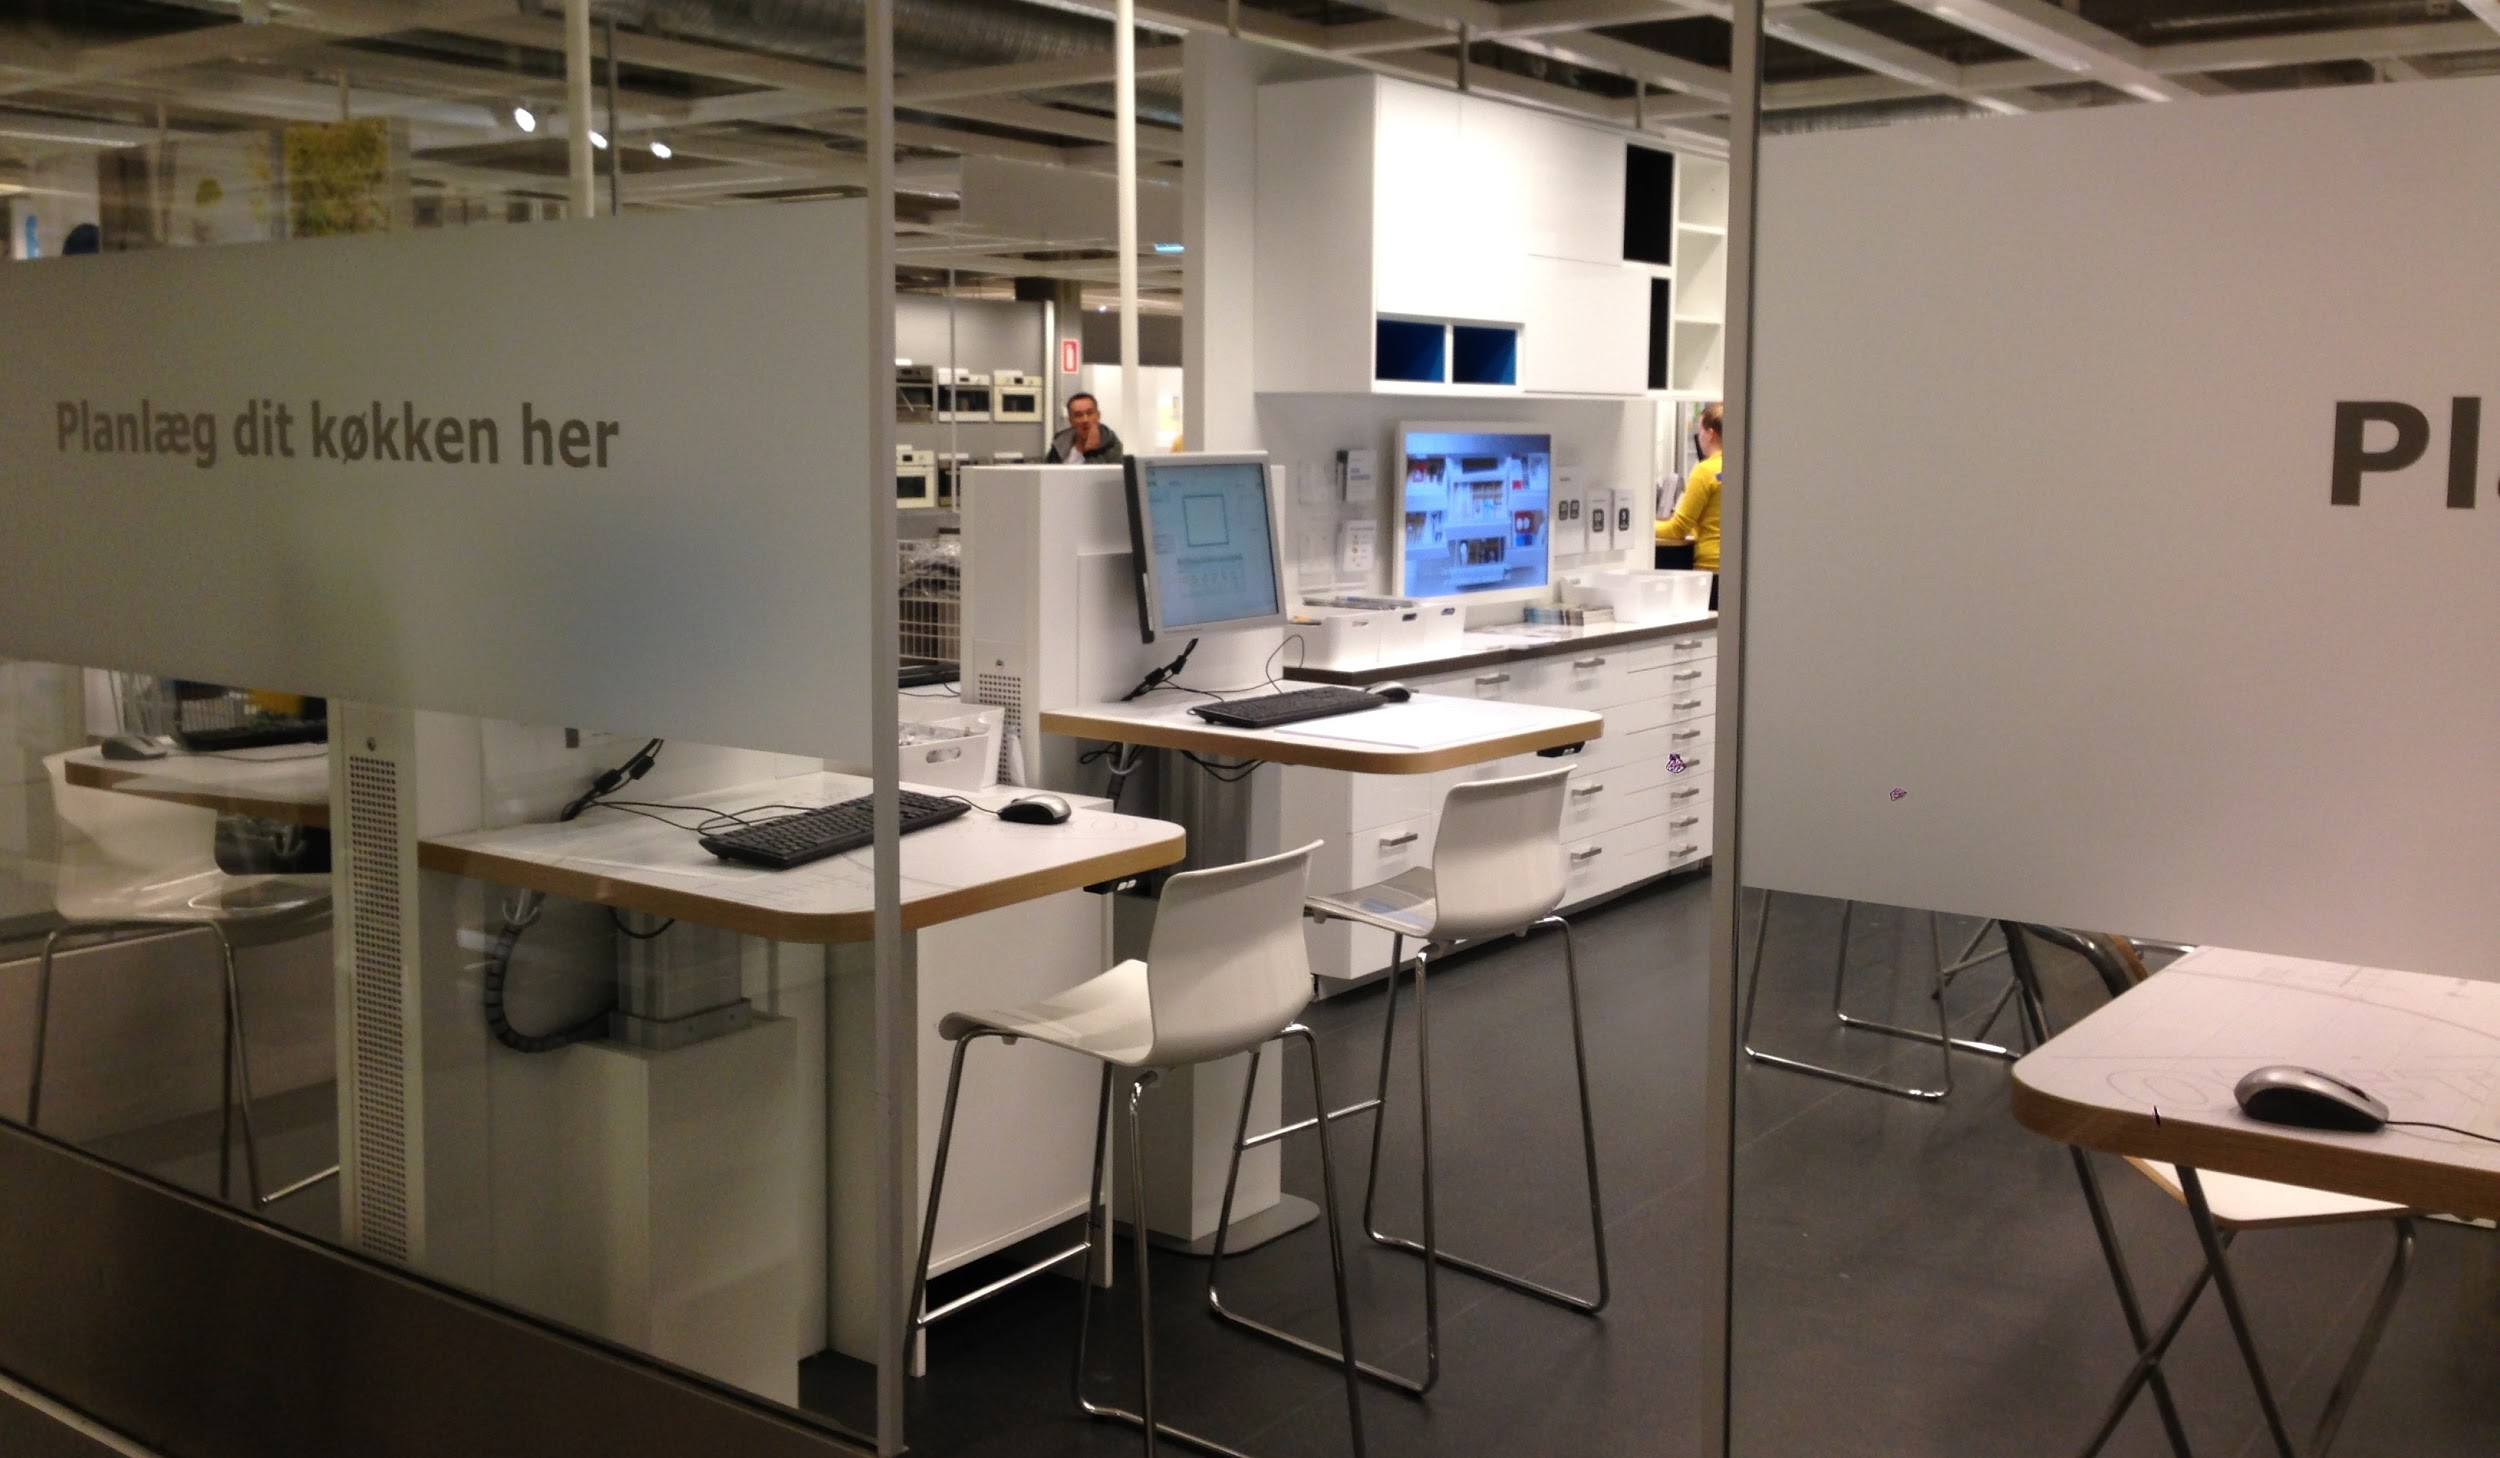
\includegraphics[scale=0.3]{kitchen3.jpg}
\caption{Picture of IKEA’s Kitchen planning app room in IKEA}
\end{figure}


This could indicate that users need help using this application. Most of the people that were asked in the initial interview also confirm that they do not use this application. Some of the participants have tried the application and know about it, but don’t use it.

The application offers plenty of useful features and can be used to give a grasp of how people’s homes would look like prior to buying the actual items, however, it is barely used by IKEA’s customers. The problem could be that the application is hard to use, leading to long time spans used to build the desired kitchen design. A solution to this possible problem could be to create an application that is more intuitive and takes less time to achieve the user’s needs.

\subsubsection{Autodesk’s “Homestyler” mobile version}

Autodesk software development company offers an application, in which the user can take or use an existing picture and modify it by adding furniture or decor to it. In the picture below you can see how 3D chair was added to an existing picture.  

\begin{figure}[H]
\centering
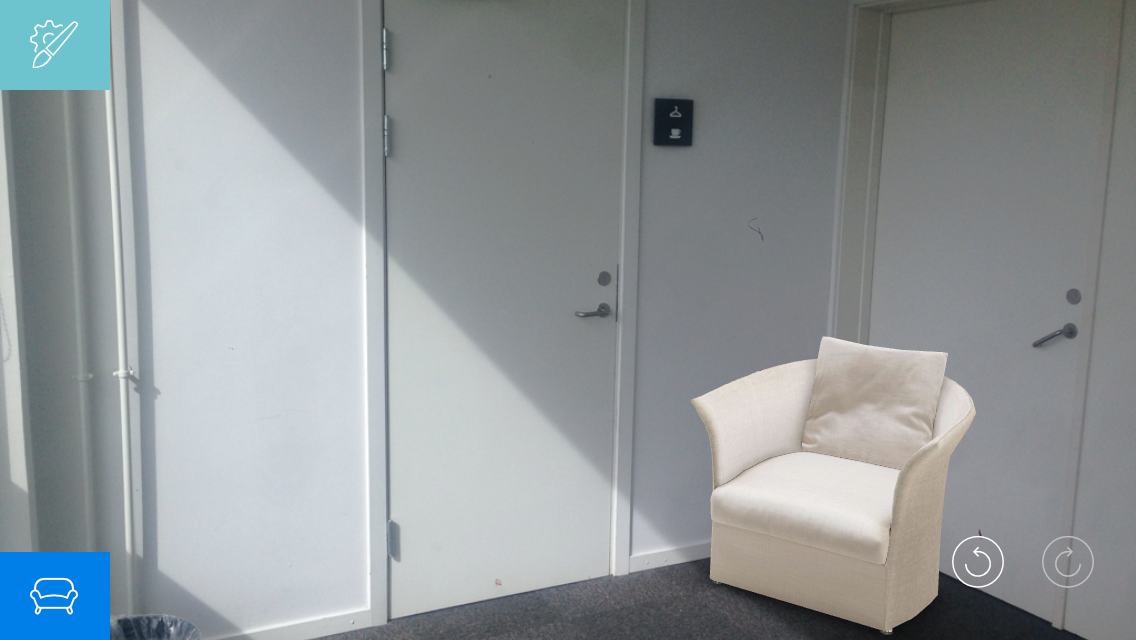
\includegraphics[scale=0.3]{homestyler1.png}
\caption{Autodesk's homestyler application}
\end{figure}

This application uses a very familiar approach of non-traditional interaction of many mobile applications, “Apple” companies’ operating systems and software. To scale a 3D object, two fingers need to be slided inwards or outwards. To rotate - two fingers need to rotate around the object, and to move the object in the environment - a simple touch-move-release action is used. This approach of controls was well designed and used by big companies so it has become the “standard” intuitive action to perform. < (source or test)

\begin{figure}[H]
\centering
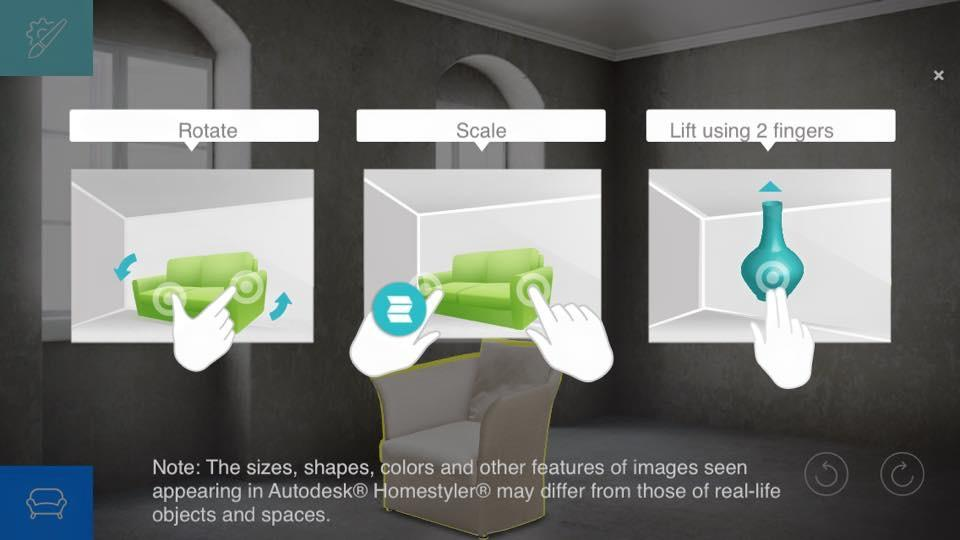
\includegraphics[scale=0.3]{homestyler2.jpg}
\caption{Autodesk's homestyler application}
\end{figure}

\subsubsection{IKEA’s Catalogue}

The Catalogue application uses “Augmented reality” (Augmented reality - webopedia.com ) principle, where 3D objects are placed on top of camera view. To make this application work, they use gyroscope to first “tag” the position of where camera is aiming, and when an object is placed, the camera can be pointed to a different direction - the object will stay at the same coordinates. Picture bellow:

\begin{figure}[H]
\centering
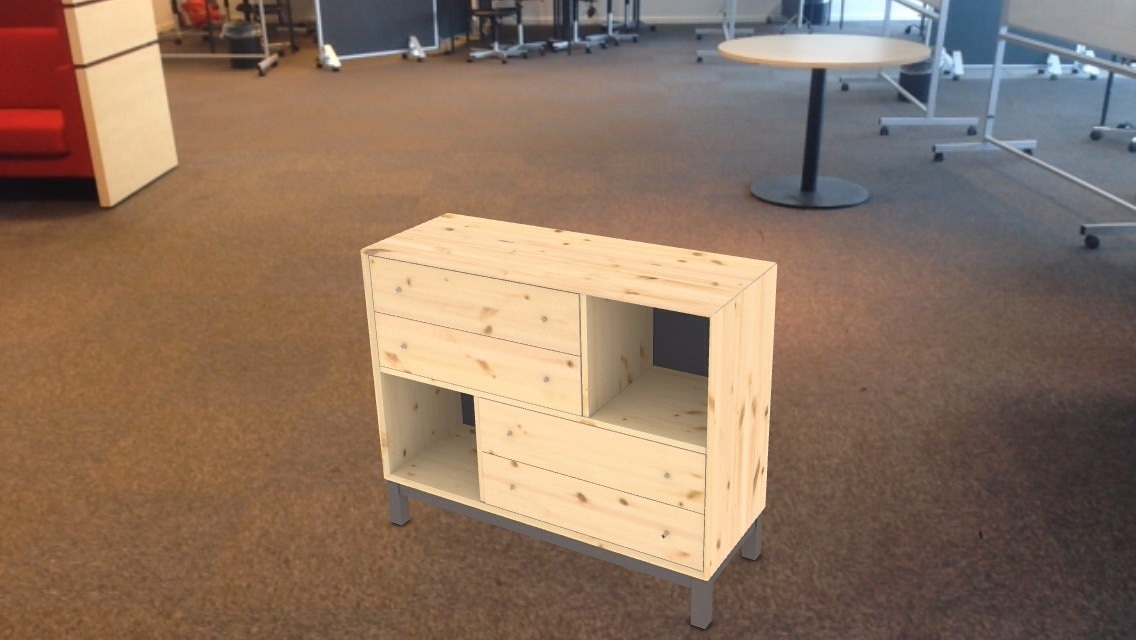
\includegraphics[scale=0.3]{catalogue1.jpg}
\caption{IKEA's Catalogues application}
\end{figure}

It is a smart way to display a 3D object in an environment, but it does not look completely well designed in this application. It is only possible to view one object from one perspective. Furthermore, the 3D object and environment have very different appearances, because the application does not do any real-time lighting calculation on the 3D object. It is also very hard to visualize the real size of the object as it does not detect nor lets the user choose its measurements.